\documentclass[12pt]{article}

\usepackage{amsmath, mathtools}
\usepackage{amsfonts}
\usepackage{amssymb}
\usepackage{graphicx}
\usepackage{colortbl}
\usepackage{xr}
\usepackage{hyperref}
\usepackage{longtable}
\usepackage{xfrac}
\usepackage{tabularx}
\usepackage{float}
\usepackage{siunitx}
\usepackage{booktabs}
\usepackage[font=small,skip=0pt]{caption}
\usepackage{caption}
\captionsetup[table]{skip=10pt}
\usepackage{pdflscape}
\usepackage{afterpage}

\usepackage{color}

\newif\ifcomments\commentstrue

\ifcomments
\newcommand{\authornote}[3]{\textcolor{#1}{[#3 ---#2]}}
\newcommand{\todo}[1]{\textcolor{red}{[TODO: #1]}}
\else
\newcommand{\authornote}[3]{}
\newcommand{\todo}[1]{}
\fi

\newcommand{\wss}[1]{\authornote{blue}{SS}{#1}} 
\newcommand{\plt}[1]{\authornote{magenta}{TPLT}{#1}} %For explanation of the template
\newcommand{\an}[1]{\authornote{cyan}{Author}{#1}}

%% Common Parts

\newcommand{\progname}{ProgName} % PUT YOUR PROGRAM NAME HERE %Every program
                                % should have a name

%\usepackage{refcheck}

\hypersetup{
    bookmarks=true,         % show bookmarks bar?
      colorlinks=true,       % false: boxed links; true: colored links
    linkcolor=red,          % color of internal links (change box color with linkbordercolor)
    citecolor=green,        % color of links to bibliography
    filecolor=magenta,      % color of file links
    urlcolor=cyan           % color of external links
}


% For easy change of table widths
\newcommand{\colZwidth}{1.0\textwidth}
\newcommand{\colAwidth}{0.13\textwidth}
\newcommand{\colBwidth}{0.82\textwidth}
\newcommand{\colCwidth}{0.1\textwidth}
\newcommand{\colDwidth}{0.05\textwidth}
\newcommand{\colEwidth}{0.8\textwidth}
\newcommand{\colFwidth}{0.17\textwidth}
\newcommand{\colGwidth}{0.5\textwidth}
\newcommand{\colHwidth}{0.28\textwidth}

% Used so that cross-references have a meaningful prefix
\newcounter{defnum} %Definition Number
\newcommand{\dthedefnum}{GD\thedefnum}
\newcommand{\dref}[1]{GD\ref{#1}}
\newcounter{datadefnum} %Datadefinition Number
\newcommand{\ddthedatadefnum}{DD\thedatadefnum}
\newcommand{\ddref}[1]{DD\ref{#1}}
\newcounter{theorynum} %Theory Number
\newcommand{\tthetheorynum}{T\thetheorynum}
\newcommand{\tref}[1]{T\ref{#1}}
\newcounter{tablenum} %Table Number
\newcommand{\tbthetablenum}{T\thetablenum}
\newcommand{\tbref}[1]{TB\ref{#1}}
\newcounter{assumpnum} %Assumption Number
\newcommand{\atheassumpnum}{P\theassumpnum}
\newcommand{\aref}[1]{A\ref{#1}}
\newcounter{goalnum} %Goal Number
\newcommand{\gthegoalnum}{P\thegoalnum}
\newcommand{\gsref}[1]{GS\ref{#1}}
\newcounter{instnum} %Instance Number
\newcommand{\itheinstnum}{IM\theinstnum}
\newcommand{\iref}[1]{IM\ref{#1}}
\newcounter{reqnum} %Requirement Number
\newcommand{\rthereqnum}{P\thereqnum}
\newcommand{\rref}[1]{R\ref{#1}}
\newcounter{nfreqnum} %NF Requirement Number
\newcommand{\rthenfreqnum}{P\thenfreqnum}
\newcommand{\nfref}[1]{NF\ref{#1}}
\newcounter{lcnum} %Likely change number
\newcommand{\lthelcnum}{LC\thelcnum}
\newcommand{\lcref}[1]{LC\ref{#1}}
\newcounter{ulcnum} %Likely change number
\newcommand{\ltheulcnum}{ULC\theulcnum}
\newcommand{\ulcref}[1]{ULC\ref{#1}}
\newcounter{typenum} %type Number
\newcommand{\rthetypenum}{P\thetypenum}
\newcommand{\tdref}[1]{TD\ref{#1}}


\usepackage{fullpage}

\begin{document}

\title{Software Requirements Specification for Mass-Mass Stoichiometry Problem} 
\author{Deemah Alomair}
\date{\today}
	
\maketitle

~\newpage

\pagenumbering{roman}

\tableofcontents

~\newpage

\section*{Revision History}

\begin{tabularx}{\textwidth}{p{3cm}p{2cm}X}
\toprule {\bf Date} & {\bf Version} & {\bf Notes}\\
\midrule
07/10/2019 & 1.0 &  First version of document\\
28/10/2019 & 2.0 &  Second version of document\\
\bottomrule
\end{tabularx}

~\newpage

\section{Reference Material}

This section records information for easy reference.

\subsection{Table of Units}

Throughout this document SI (Syst\`{e}me International d'Unit\'{e}s) is employed
as the unit system.  In addition to the basic units, several derived units are
used as described below.  For each unit, the symbol is given followed by a
description of the unit and the SI name.
~\newline

\renewcommand{\arraystretch}{1.2}
\begin{table}[ht]
  \noindent \begin{tabular}{l l l} 
    \toprule		
    \textbf{symbol} & \textbf{unit} & \textbf{SI}\\
    \midrule 
    \si{\mol} & amount of substance & mole\\
    \si{\gram} & mass	& gram\\
    \si{\gram / \mol} & molecular weight & gram/mole \\
    \si{\mol} & mole ratio & mole\\
       \bottomrule
       \hline
  \end{tabular}  
\caption{Table of Units. }

   \end{table}
  

\subsection{Table of Symbols}

The table that follows summarizes the symbols used in this document along with
their units. The choice of symbols was made to be consistent with the stoichiometry 
literature and with existing documentation for stoichiometry mass-mass program. The symbols are listed in alphabetical order.

\renewcommand{\arraystretch}{1.2}
%\noindent \begin{tabularx}{1.0\textwidth}{l l X}
\noindent \begin{longtable*}{l l p{12cm}} \toprule
\endlastfoot
\textbf{symbol} & \textbf{unit} & \textbf{description}\\
\midrule 
$m$ & \si[per-mode=symbol] {\gram} & mass.\\
$mw$ & \si[per-mode=symbol] {\gram/\mol} & molecular weight.\\ 
\bottomrule
\end{longtable*}

\subsection{Abbreviations and Acronyms}

\renewcommand{\arraystretch}{1.2}
\begin{table}[ht]
\begin{tabular}{l l} 
  \toprule		
  \textbf{symbol} & \textbf{description}\\
  \midrule 
  A & Assumption\\
  DD & Data Definition\\
  GD & General Definition\\
  GS & Goal Statement\\
  IM & Instance Model\\
  LC & Likely Change\\
  PS & Physical System Description\\
  R & Requirement\\
  SRS & Software Requirements Specification\\
 SMMP & Stoichiometry Mass-Mass Program\\
  T & Theoretical Model\\
  B & Boolean result\\
  R[0] & Reactant \\
  R1 & Reactant with known mass\\
  R2 & Reactant with unknown mass\\
  R[1] & product \\
  \bottomrule
  \end{tabular}
  \caption{ Abbreviations and Acronyms}
 \end{table}

\newpage

\pagenumbering{arabic}

\section{Introduction}

\subsection{Purpose of Document}
The purpose of this document is to describe the requirements for Stoichiometry Mass-Mass Program. A software product that will
produce a mass for unknown reactant in chemical reaction. The goal statements and theoretical models used in the SMMP code are provided, with an emphasis on explicitly identifying assumptions and unambiguous definitions. This document is intended to be used as a reference to provide ad hoc access to all information necessary to understand and verify the model. The SRS is abstract because the contents say what problem is being solved, but do not say how to solve it.\\
 This document will be used as a starting point for subsequent development phases, including writing the design specification and the software verification and validation plan. The design document will show how the requirements are to be realized, including decisions
on the numerical algorithms and programming environment. The verification and validation plan will show the steps that will be used to increase confidence in the software documentation and the implementation. Although the SRS fits in a series of documents that follow
the so-called waterfall model, the actual development process is not constrained in any way. Even when the waterfall model is not followed, as Parnas and Clements point out \cite{Parnas:Clements:1986}, the most logical way to present the documentation is still to “fake” a rational design process.


\subsection{Scope of Requirements} 

The scope of SMMP is limited to get the mass of unknown reactant in chemical reaction. 

\subsection{Characteristics of Intended Reader} \label{sec_IntendedReader}

Reviewers of this documentation should have a background on Chemistry. Especially on chemical reactions and stoichiometry.

\subsection{Organization of Document}

The organization of this document follows the template for an SRS for scientific computing software proposed by \cite{Parnas:1972} and \cite{Parnas:EAll:1984}. The presentation follows the standard pattern of presenting goals, theories, definitions, and assumptions. For readers that would like a more bottom up approach, they can start reading the instance models in Section: Instance Models and trace back to find any additional information they require. \\
The goal statements ~\ref{goals} are refined to the theoretical models and the theoretical models ~\ref{sec_theoretical} to the instance models  ~\ref{sec_instance}. 

\section{General System Description}

This section provides general information about the system.  It identifies the
interfaces between the system and its environment, describes the user
characteristics and lists the system constraints.  

\subsection{System Context}

Figure 1 shows the system context. A circle represents an external entity outside the
software, the user in this case. A rectangle represents the software system itself (SMMP).
Arrows are used to show the data flow between the system and its environment.
SMMP is mostly self-contained. The only external interaction is through the user interface. The responsibilities of the user and the system are as follows:


\begin{figure}[h!]
\begin{center}
 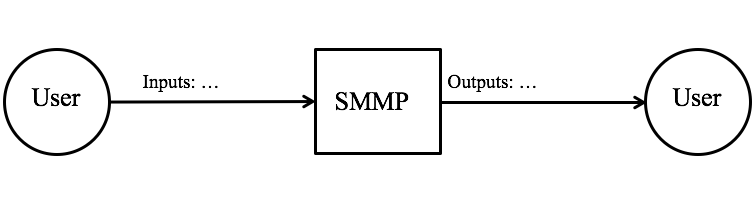
\includegraphics[width=0.9\textwidth]{SystemContextFigure}
\caption{System Context}
\label{Fig_SystemContext} 
\end{center}
\end{figure}


\begin{itemize}
\item User Responsibilities:
\begin{itemize}
\item Ensure the inputs are correct.
\item Ensure that all chemical reaction's elements entered are belong to chemical substances group.
\item Take care that consistent units are used for input variables.
\end{itemize}
\item SMMP Responsibilities:
\begin{itemize}
\item Detect data type mismatch, such as a string of characters instead of a
  floating point number.
\item Determine if the inputs satisfy the required physical and software constraints.
\item Produce an error message in case  input does not satisfy physical and software constraints.
\item Do the necessary calculations to get the final result.
\item Display the result to the end user.
\end{itemize}
\end{itemize}

\subsection{User Characteristics} \label{SecUserCharacteristics}

The end user of SMMP should have some basic knowledge on chemical stoichiometry.

\subsection{System Constraints}

There are no system constraints.

\section{Specific System Description}

This section first presents the problem description, which gives a high-level
view of the problem to be solved.  This is followed by the solution characteristics
specification, which presents the assumptions, theories, definitions and finally
the instance models.  

\subsection{Problem Description} \label{Sec_pd}

SMMP is intended to solve  Mass-Mass Stoichiometry problem in any chemical reaction. 

\subsubsection{Terminology and  Definitions}

This subsection provides a list of terms that are used in the subsequent
sections and their meaning, with the purpose of reducing ambiguity and making it
easier to correctly understand the requirements:

\begin{itemize}

\item Stoichiometry:  Is the relationship between reactants and products in chemical reactions.
\item Chemical reaction: Is a process that leads to the chemical transformation of one set of chemical substances to another.
\item Reactant: A substance that takes part in and undergoes change during a reaction.
\item Product:  Is the substance formed from chemical reactions.
\item Mole Ratio: Ratio of moles between any two compounds involved in chemical reaction.
\item Coefficients: Is the number of molecules (or atoms) involved in the reaction.
\item Molecular weight (Molar mass) :  A measure of the sum of the atomic weight values of the atoms in a molecule. 
\item Molecule: A chemical reactant or product consist of chemical element with more than one atom.
\item Compound: Molecule made up of two or more elements.
\end{itemize}

\subsubsection{Physical System Description} \label{sec_phySystDescrip}

The physical system of SMMP, as shown in Figure 2,
includes the following elements:

\begin{itemize}

\item[PS1:] Reactants mass.\\
\item[PS2:] Reactants mole ratio.\\
\item[PS3:] Reactants mole amount.\\
\item[PS4:] Reactants Molecular weight (molar mass).\\

\end{itemize}

 \begin{figure}[h!]
 \begin{center}
 {
  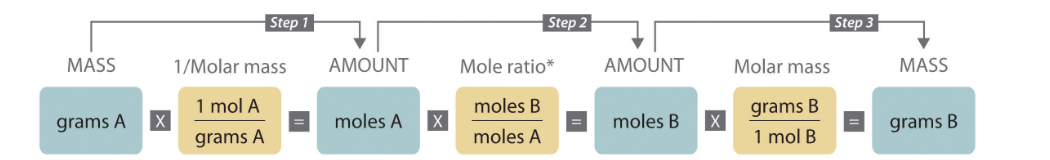
\includegraphics[width=0.9\textwidth]{physical}
 }
 \caption{\label{ Figure 2:} Physical representation of SMMP.}
 \end{center}
 \end{figure}

\subsubsection{Goal Statements}\label{goals}

\noindent Given unbalanced chemical reaction with sets of reactants and products , the goal statement are:

\begin{itemize}
\item[GS\refstepcounter{goalnum}\thegoalnum \label{G1}:] Balance the chemical reaction.
\item[GS\refstepcounter{goalnum}\thegoalnum \label{G2}:] Get the mass of one of unknown reactant.
\end{itemize}

\subsection{Solution Characteristics Specification}


The instance models that govern SMMP are presented in
Subsection~\ref{sec_instance}.  The information to understand the meaning of the
instance models and their derivation is also presented, so that the instance
models can be verified.

\subsubsection{Assumptions} \label{sec_assumpt}

This section simplifies the original problem and helps in developing the
theoretical model by filling in the missing information for the physical
system. The numbers given in the square brackets refer to the  type definition[TD], theoretical model
[T], general definition [GD], data definition [DD], instance model [IM], or
likely change [LC], in which the respective assumption is used.

\begin{itemize}

\item[A\refstepcounter{assumpnum}\theassumpnum \label{Two reactants}:] Chemical reaction with two chemical reactants.
\item[A\refstepcounter{assumpnum}\theassumpnum \label{reactant compound}:] Chemical reactant could be single element, molecule or Compound with two elements.
\item[A\refstepcounter{assumpnum}\theassumpnum \label{product compound}:] Chemical product could be single element, molecule or compound with two elements.
\item[A\refstepcounter{assumpnum}\theassumpnum \label{Known mass}:] Known mass of one chemical reactant.
\item[A\refstepcounter{assumpnum}\theassumpnum \label{Mass unit}:] Known mass entered in g unit.
\end{itemize}

\subsubsection{Type Definition}\label{Type_Detention}

This section focuses on the general variable's types that SMMP is based on.  
\begin{itemize}
\item[TD\refstepcounter{typenum}\thetypenum \label{elementT}:] ElementT = $\forall$ e $\in$ set of chemical element = 
\{ H,He,Li,Be,B,C,N,O,F,Ne,Na,Mg,Al,Si,P,S,Cl,Ar,K,
Ca,Sc,Ti,V,Cr,Mn,Fe,Co,Ni,Cu,Zn,Ga,Ge,As,Se,Br,Kr,Rb,Sr,Y,Zr,Nb,Mo,Tc,Ru,Rh,Pd,Ag,Cd,In,
Sn,Sb,Te,I,Xe,Cs,Ba,La,Ce,Pr,Nd,Pm,Sm,Eu,Gd,Tb,Dy,Ho,Er,Tm,Yb,Lu,Hf,Ta,W,Re,Os,Ir,Pt,
Au,Hg,Tl,Pb,Bi,Po,At,Rn,Fr,Ra,Ac,Th,Pa,U,Np,Pu,Am,Cm,Bk,Cf,Es,Fm,Md,No,Lr,Rf,Db,Sg,
Bh,Hs,Mt,Ds,Rg,Cn,Nh,Fl,Mc,Lv,Ts,Og \}
\item[TD\refstepcounter{typenum}\thetypenum \label{MoleculeT}:] MoleculeT = tuple of (number : $\mathbb{N}$ , element : ElementT).
\item[TD\refstepcounter{typenum}\thetypenum \label{CompoundT}:]  CompoundT =   set of MoleculeT.
\item[TD\refstepcounter{typenum}\thetypenum \label{ChemicalEqT}:] ChemicalEqT = set of (tuple of (coefficient : $\mathbb{N}$ , Compound : CompoundT))
\item[TD\refstepcounter{typenum}\thetypenum \label{ReactionT}:] ReactionT =  sequence [2] of ChemicalEq.
\end{itemize}



\subsubsection{Theoretical Models}\label{sec_theoretical}

This section focuses on the general equations and laws that SMMP is based on.  

~\newline

\noindent
\begin{minipage}{\textwidth}
\renewcommand*{\arraystretch}{1.5}
\begin{tabular}{| p{\colAwidth} | p{\colBwidth}|}
  \hline
  \rowcolor[gray]{0.9}
  Number& T\refstepcounter{theorynum}\thetheorynum \label{Mass_law}\\
  \hline
  Label&\bf Law of Conservation of Mass\\
  \hline
  Equation&  $ \sum $ mass for R =  $\sum$ mass for P.  \\
  \hline
  Description & The above equation states that there is no change in total mass occurs in a chemical reaction. The total number of    products  mass is equal to the total number of reactants mass.\\ 
   
                  \hline
  Source &
          \cite{mass_law}\\
    \hline
  Ref.\ By &  \iref{balanced}\\
  \hline
\end{tabular}
\end{minipage}\\

~\newline

\subsubsection{General Definitions}\label{sec_gendef}

N.A

\subsubsection{Data Definitions}\label{sec_datadef}


This section collects and defines all the data needed to build the instance
models. The dimension of each quantity is also given. 

~\newline


\noindent
\begin{minipage}{\textwidth}
\renewcommand*{\arraystretch}{1.5}
\begin{tabular}{| p{\colAwidth} | p{\colBwidth}|}
\hline
\rowcolor[gray]{0.9}
Number& DD\refstepcounter{datadefnum}\thedatadefnum \label{atomicMass}\\
\hline
Label& \bf Atomic Mass.\\
\hline
Symbol & -\\
\hline
% Units& $Mt^{-3}$\\
% \hline
  SI Units & -\\
  \hline
  Equation & AtomicMass: ElementT $\rightarrow$ $\mathbb{R}$ \\

  \hline
  Description &  AtomicMass(e) $\equiv$ ( e= H $\rightarrow$ 1.0079 $\vert$  e= He $\rightarrow$ 4.002 $\vert$...)  \\
   & Where e is an element $\in$ ElementT \\
   &  The function will take the element(e) and return the number of atomic mass of that element. \\ 

  \hline
  Sources& \cite{AtomicMass} \\
  \hline
  Ref.\ By & \ddref{Molecular_weight}\\
  \hline
  \end{tabular}
\end{minipage}\\

~\newline
\noindent
\begin{minipage}{\textwidth}
\renewcommand*{\arraystretch}{1.5}
\begin{tabular}{| p{\colAwidth} | p{\colBwidth}|}
\hline
\rowcolor[gray]{0.9}
Number& DD\refstepcounter{datadefnum}\thedatadefnum \label{atoms_count_m}\\
\hline
Label& \bf Count number of atoms in Molecule\\
\hline
Symbol & -\\
\hline
% Units& $Mt^{-3}$\\
% \hline
  SI Units & -\\
  \hline
  Equation & Number-of-Atoms-in-Molecule: MoleculeT  X ElementT $\rightarrow$ $\mathbb{N}$ \\

  \hline
  Description &  Number-of-Atoms-in-Molecule(m,e) $\equiv$ (m.element = e $\rightarrow$ m.number $\vert$ TRUE $\rightarrow$ 0) \\
   & Where e is an element $\in$ ElementT  \\
   &  m is an molecule  $\in$  MoleculeT \\
   &  The function will compare the molecule(m) with element(e) if they are equal it returns the number of atoms in that element else it will return 0 \\ 
  
  \hline
  Sources& \cite{Molecule:compound} \\
  \hline
  Ref.\ By &  \ddref{atoms_count_c} \\
  \hline
  \end{tabular}
\end{minipage}\\


~\newline


\noindent
\begin{minipage}{\textwidth}
\renewcommand*{\arraystretch}{1.5}
\begin{tabular}{| p{\colAwidth} | p{\colBwidth}|}
\hline
\rowcolor[gray]{0.9}
Number& DD\refstepcounter{datadefnum}\thedatadefnum \label{atoms_count_c}\\
\hline
Label& \bf Count number of atoms in compound\\
\hline
Symbol & -\\
\hline
% Units& $Mt^{-3}$\\
% \hline
  SI Units & -\\
  \hline
  Equation& Number-of-Atoms-in-Compound: CompoundT  X ElementT $\rightarrow$ $\mathbb{N}$\\
  \hline
  Description & Number-of-Atoms-in-Compound (C,e) $\equiv$ + (m : MoleculeT $\vert$ m $\in$ C $\cdot$   Number-of-Atoms-in-Molecule(m,e) ) \\
   & Where e is an element $\in$ ElementT  \\
  &  m is a molecule $\in$ C \\ 
  & C is the compound. \\ 
  & The function will take all set of molecules(m)  $\in$  compound(C)  and apply Number-of-Atoms-in-Molecule(m,e) function on them then add them together.\\
  \hline
  Sources& \cite{Molecule:compound} \\
  \hline
  Ref.\ By &  \ddref{atoms_count_Eq}\\
  \hline
  \end{tabular}
\end{minipage}\\

~\newline
\noindent
\begin{minipage}{\textwidth}
\renewcommand*{\arraystretch}{1.5}
\begin{tabular}{| p{\colAwidth} | p{\colBwidth}|}
\hline
\rowcolor[gray]{0.9}
Number& DD\refstepcounter{datadefnum}\thedatadefnum \label{atoms_count_Eq}\\
\hline
Label& \bf Count number of atoms in one side of chemical reaction\\
\hline
Symbol & -\\
\hline
% Units& $Mt^{-3}$\\
% \hline
  SI Units & -\\
  \hline
  Equation& Number-of-Atoms-in-ChemicalEq: ChemicalEqT  X ElementT $\rightarrow$ $\mathbb{N}$\\
  \hline
  Description & Number-of-Atoms-in-ChemicalEq (Ce,e) $\equiv$ + (coeff : N , C : CompoundT  $\vert$ coeff $\wedge$ C $\in$ Ce $\cdot$   Number-of-Atoms-in-Compound (C,e) $\times$ coeff) \\
  & C is the compound. \\ 
  & coeff is coefficient.\\
  & Ce is one side of chemical equation.\\
  & The function will take each  Compound(C)  $\in$  ChemicalEq(Ce)  and apply number-of-Atoms-in-Compound (C,e) function on it then multiply the result with its coefficient. The function will be applied  to all compound in ChemicalEq then add them together. \\
  \hline
  Sources&  \cite{chemicalReaction} \\
  \hline
  Ref.\ By & \ddref{balanced_reaction_elm}\\
  \hline
  \end{tabular}
\end{minipage}\\

~\newline

\noindent
\begin{minipage}{\textwidth}
\renewcommand*{\arraystretch}{1.5}
\begin{tabular}{| p{\colAwidth} | p{\colBwidth}|}
\hline
\rowcolor[gray]{0.9}
Number& DD\refstepcounter{datadefnum}\thedatadefnum \label{elements_of_compound}\\
\hline
Label& \bf Elements of a compoundT \\
\hline
Symbol & -\\
\hline
% Units& $Mt^{-3}$\\
% \hline
  SI Units & -\\
  \hline
  Equation& ElementsInCompoundT : CompoundT $\rightarrow$ set of ElementT.\\
  \hline
  Description & ElementsInCompound(C) $\equiv$ $\cup$ \{ m : MoleculeT $\vert$ m $\in$ C $\cdot$ m.element\} \\
  & where C is the compound. \\ 
  & m is Molecule $\in$ C.\\
  & The function will take each Molecule in Compound(C) and return its element then apply union to all molecules $\in$ C. \\ 
    \hline
  Sources&  \cite{Molecule:compound} \\
  \hline
  Ref.\ By & \ddref{elements_of_Eq}\\
  \hline
  \end{tabular}
\end{minipage}\\

~\newline

\noindent
\begin{minipage}{\textwidth}
\renewcommand*{\arraystretch}{1.5}
\begin{tabular}{| p{\colAwidth} | p{\colBwidth}|}
\hline
\rowcolor[gray]{0.9}
Number& DD\refstepcounter{datadefnum}\thedatadefnum \label{elements_of_Eq}\\
\hline
Label& \bf Elements of a ChemicalEq\\
\hline
Symbol & -\\
\hline
% Units& $Mt^{-3}$\\
% \hline
  SI Units & -\\
  \hline
  Equation& ElementsInChemicalEq : ChemicalEqT $\rightarrow$ set of ElementT.\\
  \hline
  Description & ElementsInChemicalEq(Ce) $\equiv$ $\cup$ \{ C : CompoundT $\vert$ C $\in$ Ce $\cdot$ ElementsInCompound(C)\} \\
  & where C is the compound $\in$ Ce. \\ 
  & ChemicalEq(Ce) is one side of chemical equation\\
  & The function will take each compound in ChemicalEq(Ce) and return its elements then apply union to all compound $\in$ Ce. \\ 
    \hline
  Sources&  \cite{chemicalReaction}\\
  \hline
  Ref.\ By & \ddref{balanced_reaction}\\
  \hline
  \end{tabular}
\end{minipage}\\

~\newline

\noindent
\begin{minipage}{\textwidth}
\renewcommand*{\arraystretch}{1.5}
\begin{tabular}{| p{\colAwidth} | p{\colBwidth}|}
\hline
\rowcolor[gray]{0.9}
Number& DD\refstepcounter{datadefnum}\thedatadefnum \label{balanced_reaction_elm}\\
\hline
Label& \bf Balanced reaction for an element \\
\hline
Symbol & -\\
\hline
% Units& $Mt^{-3}$\\
% \hline
  SI Units & -\\
  \hline
  Equation& IsBalancedReactionForElement : ReactionT x ElementT $\rightarrow$ B   \\
  \hline
  Description & IsBalancedReactionForElement (R, e) $\equiv$ Number-of-Atoms-in-ChemicalEq(R[0],e) = Number-of-Atoms-in-ChemicalEq (R[1] ,e )   \\
  & Where R[0] is the reactant on the left side of chemical reaction.\\ 
  & R[1]  is reactant on the right side of chemical reaction called "products" \\ 
  & R is a reaction\\
  & The function will take one reactant $\in$ chemical reaction  and check if it balanced or not. \\ 
  \hline
  Sources& \cite{balance}. \\
  \hline
  Ref.\ By & \ddref{balanced_reaction}\\
  \hline
  \end{tabular}
\end{minipage}\\

~\newline
\noindent
\begin{minipage}{\textwidth}
\renewcommand*{\arraystretch}{1.5}
\begin{tabular}{| p{\colAwidth} | p{\colBwidth}|}
\hline
\rowcolor[gray]{0.9}
Number& DD\refstepcounter{datadefnum}\thedatadefnum \label{balanced_reaction}\\
\hline
Label& \bf Balanced reaction  \\
\hline
Symbol & -\\
\hline
% Units& $Mt^{-3}$\\
% \hline
  SI Units & -\\
  \hline
  Equation& IsBalancedReaction : ReactionT  $\rightarrow$ B   \\
  \hline
  Description & IsBalancedReaction(R) $\equiv$ $\forall$ ( e :  ElementT $\vert$ e $\in$ ElementsInChemicalEq(R[0]) $\cdot$ IsBalancedReactionForElement(R, e))  \\
  & Where R[0] is the reactant $\in$ R.\\ 
  & R  is reaction\\ 
  & The function will take each reactant in Reaction and return if its balanced or not. if all reactants $\in$ R is balanced then R is balanced. \\ 
  \hline
  Sources& \cite{balance}. \\
  \hline
  Ref.\ By & \iref{balanced}\\
  \hline
  \end{tabular}
\end{minipage}\\

~\newline

  \noindent
\begin{minipage}{\textwidth}
\renewcommand*{\arraystretch}{1.5}
\begin{tabular}{| p{\colAwidth} | p{\colBwidth}|}
\hline
\rowcolor[gray]{0.9}
Number& DD\refstepcounter{datadefnum}\thedatadefnum \label{Coefficient}\\
\hline
Label& \bf Coefficient  \\
\hline
Symbol & -\\
\hline
% Units& $Mt^{-3}$\\
% \hline
  SI Units & -\\
  \hline
  Equation& AreAllCoefficientOnes : ChemicalEqT $\rightarrow$ B   \\
  \hline
  Description & AreAllCoefficientOnes(Ce) $\equiv$ $\forall$ ( C :  CompoundT $\vert$ C $\in$ Ce $\cdot$ Ce.coefficient =1 ) \\
  & The function will take every coefficient in compound $\in$ ChemicalEqReaction and return if its equal to 1 or not.\\ 
  &  where ChemicalEq(Ce) is one side of chemical equation\\ 
   \hline
  Sources&  \cite{Coefficients} \\
  \hline
  Ref.\ By & \iref{balanced}\\
  \hline
  \end{tabular}
\end{minipage}\\

~\newline


  \noindent
\begin{minipage}{\textwidth}
\renewcommand*{\arraystretch}{1.5}
\begin{tabular}{| p{\colAwidth} | p{\colBwidth}|}
\hline
\rowcolor[gray]{0.9}
Number& DD\refstepcounter{datadefnum}\thedatadefnum \label{Mole_ratio}\\
\hline
Label& \bf Mole ratio\\
\hline
Symbol &$ - $\\
\hline
% Units& $Mt^{-3}$\\
% \hline
  SI Units & mol \\
  \hline
  Equation& Mole ratio:  CompoundT $\rightarrow$  $\mathbb{N}$ \\
  \hline
  Description &  Mole ratio $\equiv$  	$\div$( C :  CompoundT $\vert$ C $\in$ Ce $\cdot$ Ce.coefficient )  \\
               & The above function will take the coefficient for each compound in the ChemicalEq and divide them together.  \\
                 & where  ChemicalEq(Ce) is one side of chemical reaction. \\

  \hline
  Sources& \cite{Mole_ratio}. \\
  \hline
  Ref.\ By & \iref{Mole_ratio_mole}.\\
  \hline
   \end{tabular}
\end{minipage}\\

  ~\newline
  
  \noindent
\begin{minipage}{\textwidth}
\renewcommand*{\arraystretch}{1.5}
\begin{tabular}{| p{\colAwidth} | p{\colBwidth}|}
\hline
\rowcolor[gray]{0.9}
Number& DD\refstepcounter{datadefnum}\thedatadefnum \label{Molecular_weight}\\
\hline
Label& \bf molecular weight\\
\hline
Symbol & mw\\
\hline
% Units& $Mt^{-3}$\\
% \hline
  SI Units & \si{\gram / \mol}\\
  \hline
  Equation& mw : CompoundT  $\rightarrow$ $\mathbb{R}$  \\
  \hline
  Description & mw(C) : + ( m : MoleculeT $\vert$ m $\in$ C $\cdot$ Number-of-Atoms-in-Molecule(m,e) $\times$ AtomicMass(m,e)\\
 &where $mw$ is the molecular weight of reactant .\\
 & It is computed by multiplying the AtomicMass for the molecule with the Number-of-Atoms-in-Molecule. If the reactant is compound it will take the add all its Molecule's molecular weight. \\ 
  \hline
  Sources& \cite{Molecular_weight} \\
  \hline
  Ref.\ By & \iref{Mass_mole} , \iref{Mole_mass}\\
  \hline
  \end{tabular}
\end{minipage}\\

~\newline

\subsubsection{Instance Models} \label{sec_instance}    


This section transforms the problem defined in Section~\ref{Sec_pd} into 
one which is expressed in mathematical terms. It uses concrete symbols defined 
in Section~\ref{sec_datadef} to replace the abstract symbols in the models 
identified in Sections~\ref{sec_theoretical} and~\ref{sec_gendef}.

The goals ~\ref{G1} and ~\ref{G2} are solved by ~\ref{sec_instance}.
  
~\newline

%Instance Model 1


\noindent
\begin{minipage}{\textwidth}
\renewcommand*{\arraystretch}{1.5}
\begin{tabular}{| p{\colAwidth} | p{\colBwidth}|}
  \hline
  \rowcolor[gray]{0.9}
  Number& IM\refstepcounter{instnum}\theinstnum \label{balanced}\\
  \hline
  Label& \bf balanced chemical reaction\\
  \hline
  Input& Reaction\\
  \hline
  Output& Reaction* \\
  \hline
  Description& Reaction is ReactionT such that  AreAllCoefficientOnes(R[0]) $\wedge$  AreAllCoefficientOnes(R[1])  \\
                & Reaction* is same as Reaction, but with coefficients changed such that IsBalancedReaction(R*).\\
               
  \hline
  Sources& \cite{balance}  \\
  \hline
  Ref.\ By & \gsref{G1} \\
  \hline
\end{tabular}
\end{minipage}\\
~\newline


\noindent
\begin{minipage}{\textwidth}
\renewcommand*{\arraystretch}{1.5}
\begin{tabular}{| p{\colAwidth} | p{\colBwidth}|}
  \hline
  \rowcolor[gray]{0.9}
  Number& IM\refstepcounter{instnum}\theinstnum \label{Mass_mole}\\
  \hline
  Label& \bf Converting mass to mole\\
  \hline
  Input&  m , mw \\
  \hline
  Output&  mole =  $ \frac{m}{mw} $ \\
  \hline
  Description& m is the substance mass.\\
                & mw is the substance molecular weight.\\
               & The above equation gives the amount of mole for particular substance by dividing the mass amount  with
                molecular weight. \\
  \hline
  Sources& \cite{Mass_mole} \\
  \hline
  Ref.\ By & \iref{Mole_ratio_mole}\\
  \hline
\end{tabular}
\end{minipage}\\

~\newline

\noindent
\begin{minipage}{\textwidth}
\renewcommand*{\arraystretch}{1.5}
\begin{tabular}{| p{\colAwidth} | p{\colBwidth}|}
  \hline
  \rowcolor[gray]{0.9}
  Number& IM\refstepcounter{instnum}\theinstnum \label{Mole_ratio_mole}\\
  \hline
  Label& \bf  Converting mole ratio to mole.\\
  \hline
  Input&  mole amount of R1 , mole ratio.  \\
  \hline
  Output&  mole amount of R2 = $\frac{mole-of-R1}{mole-ratio} $\\
  \hline
  Description& mol of R1 is the mole amount for known reactant.\\
                 & mole ratio is the mole ratio between R1 and R2.\\
                & The above equation gives the amount of mole for R2 substance by dividing the mole amount  of R1
                with the mole ratio. \\

  \hline
  Sources& \cite{Mole_mass/Mole_ratio_mole} \\
  \hline
  Ref.\ By & \iref{Mole_mass}\\
  \hline
\end{tabular}
\end{minipage}\\

~\newline

\noindent
\begin{minipage}{\textwidth}
\renewcommand*{\arraystretch}{1.5}
\begin{tabular}{| p{\colAwidth} | p{\colBwidth}|}
  \hline
  \rowcolor[gray]{0.9}
  Number& IM\refstepcounter{instnum}\theinstnum \label{Mole_mass}\\
  \hline
  Label& \bf  Converting mole to mass \\
  \hline
  Input&  mole amount  , mw \\
  \hline
  Output&  mass =  $ mol  \times mw  $\\
  \hline
  Description& mol is the mole amount for the substance.\\
                &  mw is the substance molecular weight.\\
               &  The above equation gives the mass  for  substance by multiplying the mole amount  
                with the molecular weight . \\
  \hline
  Sources& \cite{Mole_mass/Mole_ratio_mole} \\
  \hline
  Ref.\ By & \gsref{G2}\\
  \hline
\end{tabular}
\end{minipage}\\




\subsubsection{Input Data Constraints} \label{sec_DataConstraints}    

Table~\ref{TblInputVar} shows the data constraints on the input output
variables.  The column for physical constraints gives the physical limitations
on the range of values that can be taken by the variable.  The column for
software constraints restricts the range of inputs to reasonable values.  The
software constraints will be helpful in the design stage for picking suitable
algorithms.  The constraints are conservative, to give the user of the model the
flexibility to experiment with unusual situations.  The column of typical values
is intended to provide a feel for a common scenario.  The uncertainty column
provides an estimate of the confidence with which the physical quantities can be
measured.  This information would be part of the input if one were performing an
uncertainty quantification exercise.


\begin{table}[!h]
  \caption{Input Variables} \label{TblInputVar}
  \renewcommand{\arraystretch}{1.2}
\noindent \begin{longtable*}{l l l l c} 
  \toprule
  \textbf{Var} & \textbf{Physical Constraints} & \textbf{Software Constraints} &
                             \textbf{Typical Value} & \textbf{Uncertainty}\\
  \midrule 
      m  &  m $>$ 0  &  - & - & - \\
     
     \bottomrule
\end{longtable*}
\end{table}


\subsubsection{Properties of a Correct Solution} \label{sec_CorrectSolution}

\noindent
Table~\ref{TblOutputVar} shows the data constraints on the output variables. The column
for physical constraints gives the physical limitations on the range of values that can be
taken by the variable.

\begin{table}[!h]
\caption{Output Variables} \label{TblOutputVar}
\renewcommand{\arraystretch}{1.2}
\noindent \begin{longtable*}{l l} 
  \toprule
  \textbf{Var} & \textbf{Physical Constraints} \\
  \midrule 
  m & m $>$ 0 \\
  atoms &  $ \sum $ atoms for R[0] =  $\sum$ atoms for R[1].   \\
   \bottomrule
\end{longtable*}
\end{table}

\section{Requirements}

This section provides the functional requirements, the business tasks that the
software is expected to complete, and the nonfunctional requirements, the
qualities that the software is expected to exhibit.

\subsection{Functional Requirements}

\noindent \begin{itemize}

\item[R\refstepcounter{reqnum}\thereqnum \label{R_Inputs}:] The system will use the following inputs:\\
1- Unbalanced chemical reaction.\\
2- Mass of R1.\\

\item[R\refstepcounter{reqnum}\thereqnum \label{R_OutputInputs}:]  The system will produce the followings:\\
1- Balanced chemical reaction.
 2- Mass for R2. \\

\item[R\refstepcounter{reqnum}\thereqnum \label{R_Calculate}:] The system needs to calculate the followings:\\
1- number of atoms used in each reactant and product.\\
2- Coefficients needed for balance chemical reaction.\\
3- molecular weight for R1, R2.\\
4- Mole  amount for R1.\\
5- Mole ratio between R1 and R2.\\
6- Mole amount for R2.\\
\item[R\refstepcounter{reqnum}\thereqnum \label{R_VerifyOutput}:] The system will verify the followings:\\
1- Output is correct.\\
2-  Inputs satisfy the required physical constraints.\\
3- Mass Conservation Low applied in the chemical reaction.\\
4- No integer overflow. \\
5- Outputs satisfy the required output constraints.\\
\end{itemize}

\subsection{Nonfunctional Requirements}

This section provides the non-functional requirements, the qualities that the software is
expected to exhibit.\\

\noindent \begin{itemize}
\item[NF\refstepcounter{nfreqnum}\thenfreqnum \label{Accuracy}:]  The ability to provide a correct Solution.\\
\item[NF\refstepcounter{nfreqnum}\thenfreqnum \label{Verify}:]  The ability to test and verify the system.\\
\item[NF\refstepcounter{nfreqnum}\thenfreqnum \label{Understandability}:]  The system is understandable for novel users without any ambiguities.\\
\item[NF\refstepcounter{nfreqnum}\thenfreqnum \label{Usability}:]  The system could be used for different applications and modified easily.\\

\end{itemize}

\section{Likely Changes}    

\noindent \begin{itemize}

\item[LC\refstepcounter{lcnum}\thelcnum\label{Molecular weight}:] The system may ask the the user enter the molecular weight of the reactants.
\item[LC\refstepcounter{lcnum}\thelcnum\label{balance}:] The system may ask the user to enter balance chemical reaction.



\end{itemize}

\section{Unlikely Changes}    

\noindent \begin{itemize}

\item[ULC\refstepcounter{ulcnum}\theulcnum\label{Units}:] The units used in the system will not likely to be change.
\item[ULC\refstepcounter{ulcnum}\theulcnum\label{reactant}:] The system will not change the number of entered reactants. 

\end{itemize}

\section{Traceability Matrices and Graphs}

The purpose of the traceability matrices is to provide easy references on what
has to be additionally modified if a certain component is changed.  Every time a
component is changed, the items in the column of that component that are marked
with an ``X'' may have to be modified as well. Table~\ref{Table:A_trace} shows the dependencies of theoretical models,
general definitions, data definitions, instance models, and likely changes on
the assumptions. Table~\ref{Table:trace} shows the
dependencies of theoretical models, general definitions, data definitions, and
instance models with each other. Table~\ref{Table:R_trace} shows the
dependencies of instance models, requirements, and data constraints on each
other. 

\afterpage{
\begin{table}[h!]
\centering
\begin{tabular}{|c|c|c|c|c|c|}
\hline

	& \aref{Two reactants}&   \aref{reactant compound} &  \aref{product compound} & \aref{Known mass}& \aref{Mass unit}  \\
\hline
\tref{Mass_law}         & X& X& X& & \\ \hline
\ddref{atomicMass}         & X& X& X& & \\ \hline
\ddref{atoms_count_m}         & X& X& X& & \\ \hline
\ddref{atoms_count_c}         & X& X& X& & \\ \hline
\ddref{atoms_count_Eq}        & X& X& X& & \\ \hline
\ddref{elements_of_compound}         & X& X& X& & \\ \hline
\ddref{elements_of_Eq}          & X& X& X& & \\ \hline
\ddref{balanced_reaction_elm}          & X& X& X& & \\ \hline
\ddref{balanced_reaction}          & X& X& X& & \\ \hline
\ddref{Coefficient}          & X& X& X& & \\ \hline
\ddref{Mole_ratio}         & X& X& X& & \\ \hline
\ddref{Molecular_weight}          & X& X& X& & \\ \hline
\iref{balanced}             & X& X& X& & \\ \hline
\iref{Mass_mole}             & X& X& X& & \\ \hline
\iref{Mole_ratio_mole}            & X& X& X& & \\ \hline
\iref{Mole_mass}          & X& X& X& & \\ \hline
\rref{R_Inputs}          & X& X& X& & \\ \hline
\rref{R_OutputInputs}       & X& X& X& & \\ \hline
\rref{R_Calculate}         & X& X& X& & \\ \hline
\rref{R_VerifyOutput}      & X& X& X& & \\ \hline
\nfref{Correct}         & X& X& X& & \\ \hline
\nfref{Verify}        & X& X& X& & \\ \hline
\nfref{Understandability}         & X& X& X& & \\ \hline
\nfref{Usability}           & X& X& X& & \\ \hline
\lcref{Molecular weight}        & X& X& X& & \\ \hline
\lcref{balance}        & X& X& X& & \\ \hline
\ulcref{Units}        & X& X& X& & \\ \hline
\ulcref{reactant}        & X& X& X& & \\ \hline
\hline
\end{tabular}
\caption{Traceability Matrix Showing the Connections Between Assumptions and Other Items}
\label{Table:A_trace}
\end{table}

\newpage

\begin{table}[h!]
\centering
\begin{tabular}{|c|c|c|c|c|c|c|c|c|c|c|c|c|c|c|c|cl}
\hline        
	& \tref{Mass_law}&\ddref{atomicMass} & \ddref{atoms_count_m}& \ddref{atoms_count_c}&\ddref{atoms_count_Eq}&  \ddref{elements_of_compound} &\ddref{elements_of_Eq} & \ddref{balanced_reaction_elm} & \ddref{balanced_reaction} & \ddref{Coefficient} & \ddref{Mole_ratio} & \ddref{Molecular_weight} & \iref{balanced}& \iref{Mass_mole}& \iref{Mole_ratio_mole}& \iref{Mole_mass} \\
\hline
\tref{Mass_law}     & & & & & & X&X & & X&X & & & & & &\\ \hline
\ddref{atomicMass} & & & & & & X&X & & X&X & & & & & &\\ \hline
\ddref{atoms_count_m} & & & & & & X&X & & X&X & & & & & &\\ \hline
\ddref{atoms_count_c} & & & & & & X&X & & X&X & & & & & &\\ \hline
\ddref{atoms_count_Eq} & & & & & & X&X & & X&X & & & & & &\\ \hline
\ddref{elements_of_compound} & & & & & & X&X & & X&X & & & & & &\\ \hline
\ddref{elements_of_Eq} & & & & & & X&X & & X&X & & & & & &\\ \hline
\ddref{balanced_reaction_elm} & & & & & & X&X & & X&X & & & & & &\\ \hline
\ddref{balanced_reaction} & & & & & & X&X & & X&X & & & & & &\\ \hline
\ddref{Coefficient} & & & & & & X&X & & X&X & & & & & &\\ \hline
\ddref{Mole_ratio}  & & & & & & X&X & & X&X & & & & & &\\ \hline
\ddref{Molecular_weight} & & & & & & X&X & & X&X & & & & & &\\ \hline
\iref{balanced} & & & & & & X&X & & X&X & & & & & &\\ \hline
\iref{Mass_mole}      & & & & & & X&X & & X&X & & & & & &\\ \hline
\iref{Mole_ratio_mole}    & & & & & & X&X & & X&X & & & & & &\\ \hline
\iref{Mole_mass}    & & & & & & X&X & & X&X & & & & & &\\ \hline
\hline
\end{tabular}
\caption{Traceability Matrix Showing the Connections Between Items of Different Sections}
\label{Table:trace}
\end{table}

\begin{table}[h!]
\centering
\begin{tabular}{|c|c|c|c|c|c|c|c|c|c|c|}
\hline
	& \iref{balanced} & \iref{Mass_mole}& \iref{Mole_ratio_mole}& \iref{Mole_mass} & \ref{sec_DataConstraints}& \rref{R_Inputs}& \rref{R_OutputInputs} & \rref{R_Calculate} & \rref{R_VerifyOutput} \\
\hline
\iref{balanced}  & & & X& X&X & X& X& X& X \\ \hline
\iref{Mass_mole}            & & & X&X & X& X&X & X&  \\ \hline
\iref{Mole_ratio_mole}     & & & & X& & &X &X &  \\ \hline
\iref{Mole_mass}             & & & & &X & &X & X& \\ \hline
\rref{R_Inputs}                &X & X&X &X & X& & X& X&X  \\ \hline
\rref{R_OutputInputs}    & & & & & X& X& & X&X  \\ \hline
\rref{R_Calculate}    & & & X& X&X X& X& & &X  \\ \hline
\rref{R_VerifyOutput}   & & & & & & & X&X & \\ \hline
\hline
\end{tabular}
\caption{Traceability Matrix Showing the Connections Between Requirements and Instance Models}
\label{Table:R_trace}
\end{table}
}
\newpage

\section{Values of Auxiliary Constants}
NA 

\newpage
\bibliographystyle{unsrt}
\bibliography {../../ReferenceMaterial/References}

\newpage
\end{document}
